\documentclass{article}
\usepackage[utf8]{inputenc}
\usepackage[margin=1in]{geometry}
\usepackage{soul,color}
\usepackage{amsfonts, amsmath}
\usepackage{bbm}
\usepackage{enumitem}
\usepackage[nobreak=true]{mdframed}
\usepackage{amssymb}
\usepackage{graphicx}

\newcommand{\solution}{\textbf{Solution: }}
\newcommand{\N}{\mathcal{N}}
% \newcommand{\Pbf}{\textbf{P}}
\newcommand{\R}{\mathbb{R}}
\newcommand{\E}{\mathbb{E}}
\newcommand{\Var}{\text{Var}}
\newcommand{\Cov}{\text{Cov}}
\newcommand{\Ell}{\mathcal{L}}
\DeclareMathOperator*{\argmin}{argmin}

\usepackage[utf8]{inputenc}

% Default fixed font does not support bold face
\DeclareFixedFont{\ttb}{T1}{txtt}{bx}{n}{8} % for bold
\DeclareFixedFont{\ttm}{T1}{txtt}{m}{n}{8}  % for normal

% Custom colors
\usepackage{color}
\definecolor{deepblue}{rgb}{0,0,0.5}
\definecolor{deepred}{rgb}{0.6,0,0}
\definecolor{deepgreen}{rgb}{0,0.5,0}

\usepackage{listings}

% Python style for highlighting
\newcommand\pythonstyle{\lstset{
language=Python,
basicstyle=\ttfamily\footnotesize,
otherkeywords={self},             % Add keywords here
keywordstyle=\ttb\color{deepblue},
emph={MyClass,__init__},          % Custom highlighting
emphstyle=\ttb\color{deepred},    % Custom highlighting style
stringstyle=\color{deepgreen},
frame=tb,                         % Any extra options here
showstringspaces=false           % 
}}


% Python environment
\lstnewenvironment{python}[1][]
{
\pythonstyle
\lstset{#1}
}
{}

% Python for external files
\newcommand\pythonexternal[2][]{{
\pythonstyle
\lstinputlisting[#1]{#2}}}

% Python for inline
\newcommand\pythoninline[1]{{\pythonstyle\lstinline!#1!}}

\title{CS189, HW5: Decision Trees}
\author{ Completed by: Matthew Wu}
% \date{January 2017}
\date{}

\begin{document}

\maketitle

\subsection*{1. Decision Tree Implementation}
The following code was used to implement decision trees:

\begin{python}
import numpy as np
from collections import Counter
import math

class DecisionTree(object):
    def __init__(self, categorical_vars = set(), max_depth = float('inf'), m = None):
        self.categorical_vars = categorical_vars
        self.max_depth = max_depth
        self.m = m

    class Node(object):
        def __init__(self, myTree, points, depth = 0):
            self.myTree = myTree
            self.is_leaf = False
            self.points = points
            self.depth = depth
            if self.should_stop():
                self.stop()
                return
            best_feature, best_split = myTree.segmenter(points)
            if best_feature == None:
                self.stop()
                return
            self.split_rule = (best_feature, best_split)
            left_points = []
            right_points = []
            if best_feature in myTree.categorical_vars:
                for p in points:
                    if self.myTree.data[p][best_feature] == best_split:
                        left_points.append(p)
                    else:
                        right_points.append(p)
            else:
                for p in points:
                    if self.myTree.data[p][best_feature] < best_split:
                        left_points.append(p)
                    else:
                        right_points.append(p)
            self.left = myTree.Node(self.myTree, left_points, depth + 1)
            self.right = myTree.Node(self.myTree, right_points, depth + 1)

        def should_stop(self):
            if self.depth >= self.myTree.max_depth:
                return True
            label = None
            for p in self.points:
                if not label:
                    label = self.myTree.labels[p]
                    continue
                if self.myTree.labels[p] != label:
                    return False
            return True

        def stop(self):
            frequencies = {}
            for p in self.points:
                l = float(self.myTree.labels[p])
                if l in frequencies:
                    frequencies[l] += 1
                else:
                    frequencies[l] = 1
            self.label = max(frequencies, key=frequencies.get)
            self.is_leaf = True

        def classify(self, point):
            if self.is_leaf:
                return self.label
            feature, split = self.split_rule
            if feature in self.myTree.categorical_vars:
                if point[feature] == split:
                    return self.left.classify(point)
                return self.right.classify(point)
            else:
                if point[feature] < split:
                    return self.left.classify(point)
                return self.right.classify(point)

        def get_path(self, point):
            if self.is_leaf:
                return [(self.label,)]
            feature, split = self.split_rule
            if feature in self.myTree.categorical_vars:
                if point[feature] == split:
                    return [(feature, split, "is")] + self.left.get_path(point)
                return [(feature, split, "isn't")] + self.right.get_path(point)
            else:
                if point[feature] < split:
                    return [(feature, split, "<")] + self.left.get_path(point)
                return [(feature, split, ">=")] + self.right.get_path(point)

        def decision_list(self):
            if self.is_leaf:
                return self.label
            left_lst = self.left.decision_list()
            right_lst = self.right.decision_list()
            return [self.split_rule, [left_lst, right_lst]]

    def train(self, data, labels, points=None):
        self.data = data
        self.labels = labels
        self.num_features = data.shape[1]
        if self.m == None:
            self.m = math.ceil(self.num_features**.5)
        if not points:
            points = [i for i in range(data.shape[0])]
        self.root = self.Node(self, points)

    def segmenter(self, points):
        total_labels = 0
        zero_labels = 0
        for p in points:
            if self.labels[p] == 0:
                zero_labels += 1
            total_labels += 1

        def find_split_for_feature(feature):
            best_entropy = float('inf')
            best_split = None
            if feature not in self.categorical_vars:
                left_zero_labels = 0
                left_total_labels = 0
                sorted_points = sorted(points, key=lambda p: self.data[p][feature])
                previous_value = self.data[sorted_points[0]][feature]
                if self.labels[sorted_points[0]] == 0:
                    left_zero_labels += 1
                left_total_labels += 1
                for i in range(1, len(sorted_points)):
                    new_value = self.data[sorted_points[i]][feature]
                    if previous_value != new_value:
                        new_entropy = self.impurity(
                            left_zero_labels,
                            left_total_labels - left_zero_labels,
                            zero_labels - left_zero_labels,
                            total_labels - left_total_labels - zero_labels + left_zero_labels)
                        if new_entropy < best_entropy:
                            best_entropy = new_entropy
                            best_split = (previous_value + new_value) / 2
                    previous_value = new_value
                    if self.labels[sorted_points[i]] == 0:
                        left_zero_labels += 1
                    left_total_labels += 1
            else:
                cat_total_freq = Counter()
                cat_zero_freq = Counter()
                for p in points:
                    category = self.data[p][feature]
                    label = self.labels[p]
                    cat_total_freq[category] += 1
                    if label == 0:
                        cat_zero_freq[category] += 1
                for category in cat_total_freq:
                    left_total_labels = cat_total_freq[category]
                    left_zero_labels = cat_zero_freq[category]
                    new_entropy = self.impurity(
                        left_zero_labels,
                        left_total_labels - left_zero_labels,
                        zero_labels - left_zero_labels,
                        total_labels - left_total_labels - zero_labels + left_zero_labels)
                    if new_entropy < best_entropy:
                        best_entropy = new_entropy
                        best_split = category
            return best_entropy, best_split

        #Pick random features to split on
        possible_split_features = self.select_random_features()
        best_entropy = float('inf')
        best_split = None
        best_feature = None
        for feature in possible_split_features:
            new_entropy, new_split = find_split_for_feature(feature)
            if new_entropy < best_entropy:
                best_entropy = new_entropy
                best_split = new_split
                best_feature = feature
        return best_feature, best_split

    def impurity(self, left_zeros, left_ones, right_zeros, right_ones):
        def H(prob):
            if prob == 0 or prob == 1:
                return 0
            return - prob * np.log2(prob) - (1 - prob) * np.log2(1 - prob)
        left_total = left_zeros + left_ones
        right_total = right_zeros + right_ones
        if left_total == 0 or right_total == 0:
            return float('inf')
        left_prob_zero = left_zeros / left_total
        right_prob_zero = right_zeros / right_total
        left_weight = left_total / (left_total + right_total)
        right_weight = 1 - left_weight
        return H(left_prob_zero) * left_weight + H(right_prob_zero) * right_weight

    def select_random_features(self):
        lst = [i for i in range(self.num_features)]
        np.random.shuffle(lst)
        return lst[:self.m]

    def predict(self, data):
        return self.root.classify(data)

    def get_first_split(self):
        return self.root.split_rule

    def get_path(self, data):
        return self.root.get_path(data)

    def get_decision_list(self):
        return self.root.decision_list()

\end{python}

\newpage

\subsection*{2. Random Forest Implementation}
The following code was used to implement random forests:

\begin{python}
import numpy as np
import math
from collections import Counter
from DecisionTree import DecisionTree
import sys

class RandomForest(object):
    def __init__(self, num_trees, num_sample_points = None,
        categorical_vars=set(), max_depth=float('inf'), m = None):
        self.num_trees = num_trees
        self.num_sample_points = num_sample_points
        self.categorical_vars = categorical_vars
        self.max_depth = max_depth
        self.m = m

    def train(self, data, labels):
        self.data = data
        self.labels = labels
        self.num_features = data.shape[1]
        self.N = data.shape[0]
        if self.num_sample_points == None:
            self.num_sample_points = self.N
        if self.m == None:
            self.m = math.ceil(self.num_features**.5)
        self.trees = []
        for i in range(self.num_trees):
            points = self.draw_sample()
            new_tree = DecisionTree(self.categorical_vars, self.max_depth, self.m)
            new_tree.train(self.data, self.labels, points)
            self.trees.append(new_tree)
            #print("Finished training tree " + str(i + 1))
            #sys.stdout.flush()

    def predict(self, data):
        counts = Counter()
        for tree in self.trees:
            prediction = tree.predict(data)
            counts[prediction] += 1
        prediction = max(counts, key=counts.get)
        return prediction

    def most_frequent_first_splits(self):
        counts = Counter()
        for tree in self.trees:
            split = tree.get_first_split()
            counts[split] += 1
        lst = sorted(counts, key=counts.get)
        return [(i, counts[i]) for i in lst][::-1]

    def draw_sample(self):
        return [np.random.randint(self.N) for i in range(self.num_sample_points)]
\end{python}

\newpage

\subsection*{3. Implementation Details}
\begin{enumerate}[label=\alph*)]
\item
For categorical features, the possible splits I tried were all of the samples with the same category separated from all the samples with any category besides that one.\\
For missing values, I replaced the missing values with the mean of the other sample points if it was continuous, or the most frequent category if it was categorical.
\item
The stopping criteria were if all of the labels in a node were the same, if the node was at the maximum depth, or if there were no good splits (e.g. two sample points are at the same point in $d$-dimensional space but they have different labels).
\item
I implemented the algorithm that sorts the sample points for splitting them into the left and right nodes as discussed in lecture. I also reduced memory usage (which probably increases speed too) by only keeping one matrix of sample points, and referring to that one matrix with pointers. Every node keeps track of a list of points to the data.
\item
I implemented random forests by using bagging to select sample points with replacement for each of $N$ decision trees, where $N$ is a parameter that is passed in to the random forest. The random forest classifies points by a majority vote from the decision trees.
\end{enumerate}

\newpage

\subsection*{4. Performance Evaluation}

The following table shows the classification accuracy for the decision trees and random forests, for both training and validation data, for all three training sets.
\vspace{.25in}
\begin{center}
Classification Accuracy\\
\begin{tabular}{|c|c|c|c|}
\hline
 & Spam & Census & Titanic \\
\hline
Decision Tree Training & 98.809\% & 85.752\% & 84.588\% \\
Decision Tree Validation & 80.169\% & 84.979\% & 77.181\% \\
\hline
Random Forest Training & 99.737\% & 86.646\% & 84.941\%	 \\
Random Forest Validation & 90.127\% & 85.895\% & 83.221\% \\
\hline
\end{tabular}\\
\vspace{.5in}
Hyperparameters\\
\begin{tabular}{|c|c|c|c|}
\hline
 & Spam & Census & Titanic \\
\hline
Decision Tree & Max Depth: 25 & Max Depth: 10 & Max Depth: 7 \\
\hline
Random Forest & Trees: 25 & Trees: 25 & Trees: 250 \\
\hline
\end{tabular}
\end{center}

\newpage

\subsection*{5. Spam Data Set}
\begin{enumerate}[label=\alph*)]
\item
I implemented a bag of words with 256 features. The first 128 features is the raw count of the frequency of the words in each of 128 buckets. The last 128 features
is the normalized count of the frequency of the words in each of 128 buckets.

\item
The method I described above isn't interpretable, so for the next two sections I just used the default featurizer given to us.
\begin{python}
money < 0.5
! < 0.5
volumes < 0.5
meter < 0.5
path < 0.5
& >= 0.5
width < 1.0
private < 0.5
pain < 1.0
out < 0.5
Therefore this email is ham

money < 0.5
! >= 0.5
( < 0.5
prescription >= 0.5
other < 1.5
Therefore this email is spam
\end{python}

\item
I generated 100 trees and listed the four most frequent splits below.\\
! $<$ 0.5 (22 trees)\\
meter $<$ 0.5 (15 trees)\\
money $<$ 0.5 (12 trees)\\
prescription $<$ 0.5 (9 trees)\\

\end{enumerate}

\newpage

\subsection*{6. Census Data Set}
\begin{enumerate}[label=\alph*)]
\item
The only transformations I performed on the data involved filling in missing values with the mean for continuous features or the most frequently occurring category for the categorical data.
\item
capital-gain $<$ 5119.0\\
relationship isn't Husband\\
occupation isn't Prof-specialty\\
marital-status is Married-civ-spouse\\
education isn't Bachelors\\
capital-loss $<$ 1794.0\\
education isn't Masters\\
occupation isn't Exec-managerial\\
sex isn't Male\\
occupation isn't Adm-clerical\\
Therefore this person makes less than \$50k\\

capital-gain $>=$ 5119.0\\
marital-status is Married-civ-spouse\\
occupation isn't Farming-fishing\\
hours-per-week $>=$ 22.0\\
hours-per-week $>=$ 50.5\\
Therefore this person makes more than \$50k\\

\item
I generated 100 trees and listed the four most frequent splits below.\\
marital-status is Married-civ-spouse (38 trees)\\
relationship is Husband (17 trees)\\
capital-gain $<$ 7055.5 (9 trees)\\
age $<$ 28.5 (8 trees)
\newpage
\item

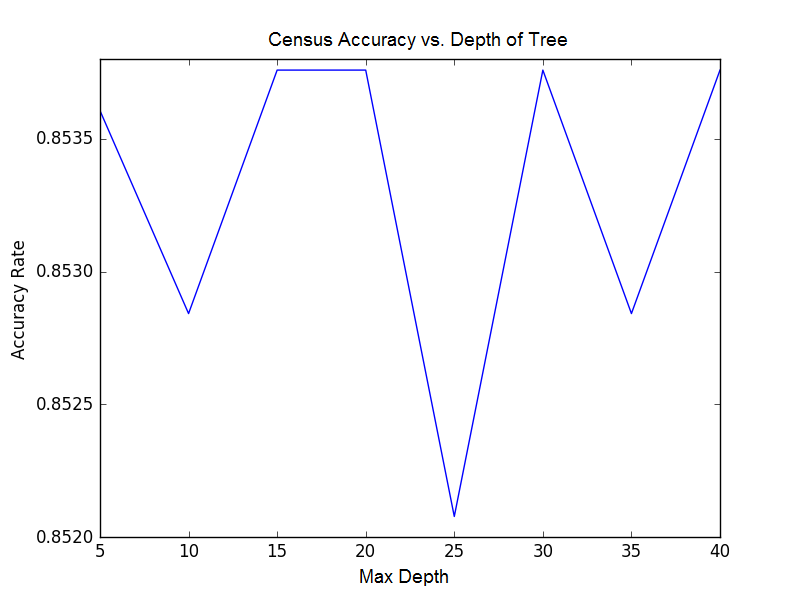
\includegraphics[scale=.6]{figure_1.png}\\
Lots of variance still occurs with just 1 tree, regardless of its maximum depth. A random forest is more effective in classification than just increasing the depth.

\end{enumerate}
\newpage
\subsection*{7. Titanic Data Set}
Because the tree is so shallow, some of the splits don't appear to do anything, but may prove themselves useful if the tree were greater than depth three.
\begin{python}
sex is male
    age < 9.5
        sibsp < 2.0
            survived
        sibsp >= 2.0
            died
    age >= 9.5
        pclass < 1.5
            died
        pclass >= 1.5
            died
sex isnt male
    pclass < 2.5
        age < 59.0
            survived
        age >= 59.0
            survived
    pclass >= 2.5
        fare < 35.5375
            survived
        fare >= 35.5375
            died
\end{python}

\newpage

\subsection*{Appendix}
The following code was used for Titanic:
\begin{python}
import numpy as np
import scipy.io
import csv
from sklearn.feature_extraction import DictVectorizer
from sklearn.preprocessing import Imputer
import sys
from DecisionTree import DecisionTree
from RandomForest import RandomForest
from collections import Counter
import math

TRAINING_FRACTION = .85

train_filename = 'hw5_titanic_dist/titanic_training.csv'
test_filename = 'hw5_titanic_dist/titanic_testing_data.csv'

training_data = []
testing_data = []

with open(train_filename) as csvfile:
    reader = csv.DictReader(csvfile)
    for row in reader:
        training_data.append(row)

with open(test_filename) as csvfile:
    reader = csv.DictReader(csvfile)
    for row in reader:
        testing_data.append(row)

i = 0
while i < len(training_data):
    data = training_data[i]
    if data['survived'] == '':
        del training_data[i]
        continue
    del data['ticket']
    del data['cabin']
    for key in data:
        try:
            data[key] = float(data[key])
        except:
            if data[key] == '':
                data[key] = np.nan
            continue
    i += 1

i = 0
while i < len(testing_data):
    data = testing_data[i]
    del data['ticket']
    del data['cabin']
    for key in data:
        try:
            data[key] = float(data[key])
        except:
            if data[key] == '':
                data[key] = np.nan
            continue
    i += 1

labels = np.array([[sample['survived']] for sample in training_data])

all_data = training_data + testing_data

continuous_data = np.array([[sample['pclass'], sample['age'],
    sample['sibsp'], sample['parch'], sample['fare']] for sample in all_data])

V = Imputer()
continuous_data = V.fit_transform(continuous_data)

categorical_data = [[sample['sex'], sample['embarked']] for sample in all_data]

#Use the most frequent occurence to replace blanks in categorical data
num_cat_rows = len(categorical_data)
num_cat_feat = len(categorical_data[0])

for col in range(num_cat_feat):
    counts = Counter()
    impute = False
    for row in range(num_cat_rows):
        val = categorical_data[row][col]
        if val != np.nan:
            counts[val] += 1
        else:
            impute = True
    if impute:
        new_val = max(counts, key=counts.get)
        for row in range(num_cat_rows):
            if categorical_data[row][col] == np.nan:
                categorical_data[row][col] = new_val

#Convert categorical data into floats
translation_list = []
inverse_list = []
for col in range(num_cat_feat):
    translator = {}
    inverse = {}
    i = 1
    for row in range(num_cat_rows):
        val = categorical_data[row][col]
        if val in translator:
            categorical_data[row][col] = translator[val]
        else:
            translator[val] = float(i)
            categorical_data[row][col] = translator[val]
            inverse[i] = val
            i += 1
    translation_list.append(translator)
    inverse_list.append(inverse)

categorical_data = np.array(categorical_data)

TRAIN_SIZE = len(training_data)
TEST_SIZE = len(testing_data)
CONTINUOUS_FEATURES = continuous_data.shape[1]
CATEGORICAL_FEATURES = categorical_data.shape[1]
NUM_FEATURES = CONTINUOUS_FEATURES + CATEGORICAL_FEATURES

all_data = np.hstack((continuous_data, categorical_data))
traindata = all_data[:TRAIN_SIZE]
testing_data = all_data[TRAIN_SIZE:]

#Shuffling the data and setting aside a validation set
traindata = np.append(traindata, labels, axis=1)
np.random.shuffle(traindata)

SIZE = traindata.shape[0]

N = math.ceil(SIZE * TRAINING_FRACTION)

traindata, labels = traindata[:,:-1], traindata[:, -1:]

training_data = traindata[:N]
training_labels = labels[:N]
validation_data = traindata[N:]
validation_labels = labels[N:]

num_training_points = N
num_validation_points = validation_data.shape[0]
#Validation set end

cat_set = set([5, 6])

def classify_with_decision_tree():
    tree = DecisionTree(max_depth = 7, categorical_vars = cat_set)
    tree.train(training_data, training_labels)

    num_right = 0
    for i in range(num_training_points):
        prediction = tree.predict(training_data[i])
        if prediction == training_labels[i]:
            num_right += 1
    print("Training Accuracy: " + str(num_right / num_training_points))

    num_right = 0
    for i in range(num_validation_points):
        prediction = tree.predict(validation_data[i])
        if prediction == validation_labels[i]:
            num_right += 1
    print("Validation Accuracy: " + str(num_right / num_validation_points))

def classify_with_random_forest():
    forest = RandomForest(num_trees = 250, max_depth = 7, categorical_vars = cat_set)
    forest.train(training_data, training_labels)

    num_right = 0
    for i in range(num_training_points):
        prediction = forest.predict(training_data[i])
        if prediction == training_labels[i]:
            num_right += 1
    print("Training Accuracy: " + str(num_right / num_training_points))

    num_right = 0
    for i in range(num_validation_points):
        prediction = forest.predict(validation_data[i])
        if prediction == validation_labels[i]:
            num_right += 1
    print("Validation Accuracy: " + str(num_right / num_validation_points))

feature_names = ['pclass', 'age', 'sibsp', 'parch', 'fare', 'sex', 'embarked']

def output_tree():
    tree = DecisionTree(max_depth = 3, categorical_vars = cat_set)
    tree.train(training_data, training_labels)
    lst = tree.get_decision_list()

    def output_node(lst, depth=0):
        if type(lst) == list:
            feature, value = lst[0]
            left, right = ' < ', ' >= '
            if feature in cat_set:
                value = inverse_list[feature - CONTINUOUS_FEATURES][value]
                left, right = ' is ', " isn't "
            name = feature_names[feature]
            print('    ' * depth + name + left + str(value))
            output_node(lst[1][0], depth + 1)
            print('    ' * depth + name + right + str(value))
            output_node(lst[1][1], depth + 1)
        else:
            label = 'survived' if lst == 1 else 'died'
            print('    ' * depth + label)

    output_node(lst)

def predict_test_data():
    forest = RandomForest(num_trees = 250, max_depth = 7, categorical_vars = cat_set)
    forest.train(training_data, training_labels)

    num_right = 0
    for i in range(num_training_points):
        prediction = forest.predict(training_data[i])
        if prediction == training_labels[i]:
            num_right += 1
    print("Training Accuracy: " + str(num_right / num_training_points))

    num_right = 0
    for i in range(num_validation_points):
        prediction = forest.predict(validation_data[i])
        if prediction == validation_labels[i]:
            num_right += 1
    print("Validation Accuracy: " + str(num_right / num_validation_points))

    guesses = []
    for i in range(TEST_SIZE):
        point = testing_data[i]
        guess = tree.predict(point)
        guesses.append(int(guess))

    with open('titanic_1.csv', 'w', newline='') as csvfile:
        writer = csv.writer(csvfile)
        writer.writerow(['Id', 'Category'])
        i = 1
        for g in guesses:
            writer.writerow([i, g])
            i += 1

#classify_with_decision_tree()
#classify_with_random_forest()
#output_tree()
#predict_test_data()
\end{python}

\newpage

The following code was used for Spam:
\begin{python}
import numpy as np
import scipy.io
import matplotlib.pyplot as plt
import csv
import math
import sys
from DecisionTree import DecisionTree
from RandomForest import RandomForest

#traindatafilename = "hw5_spam_dist/dist/spam_data"
traindatafilename = 'hw5_spam_dist/dist/default_spam_data'

data = scipy.io.loadmat(traindatafilename)

traindata = data['training_data']
NUM_FEATURES = traindata.shape[1]
testdata = data['test_data']
labels = data['training_labels']
labels = labels.transpose()
traindata = np.append(traindata, labels, axis=1)
np.random.shuffle(traindata)

SIZE = traindata.shape[0]

TRAINING_FRACTION = .9

N = math.ceil(SIZE * TRAINING_FRACTION)

traindata, labels = traindata[:,:-1], traindata[:, -1:]

training_data = traindata[:N]
training_labels = labels[:N]
validation_data = traindata[N:]
validation_labels = labels[N:]

num_training_points = N
num_validation_points = validation_data.shape[0]

def classify_with_decision_tree():
    tree = DecisionTree(max_depth = 25)
    tree.train(training_data, training_labels)

    num_right = 0
    for i in range(num_training_points):
        prediction = tree.predict(training_data[i])
        if prediction == training_labels[i]:
            num_right += 1
    print("Training Accuracy: " + str(num_right / num_training_points))

    num_right = 0
    for i in range(num_validation_points):
        prediction = tree.predict(validation_data[i])
        if prediction == validation_labels[i]:
            num_right += 1
    print("Validation Accuracy: " + str(num_right / num_validation_points))

def classify_with_random_forest():
    forest = RandomForest(num_trees = 25, max_depth = 25)
    forest.train(training_data, training_labels)

    num_right = 0
    for i in range(num_training_points):
        prediction = forest.predict(training_data[i])
        if prediction == training_labels[i]:
            num_right += 1
    print("Training Accuracy: " + str(num_right / num_training_points))

    num_right = 0
    for i in range(num_validation_points):
        prediction = forest.predict(validation_data[i])
        if prediction == validation_labels[i]:
            num_right += 1
    print("Validation Accuracy: " + str(num_right / num_validation_points))

def predict_test_data():
    forest = RandomForest(num_trees = 25, max_depth = 25)
    forest.train(training_data, training_labels)

    num_right = 0
    for i in range(num_training_points):
        prediction = forest.predict(training_data[i])
        if prediction == training_labels[i]:
            num_right += 1
    print("Training Accuracy: " + str(num_right / num_training_points))

    num_right = 0
    for i in range(num_validation_points):
        prediction = forest.predict(validation_data[i])
        if prediction == validation_labels[i]:
            num_right += 1
    print("Validation Accuracy: " + str(num_right / num_validation_points))

    guesses = []
    for i in range(testdata.shape[0]):
        point = testdata[i]
        guess = forest.predict(point)
        guesses.append(int(guess))

    with open('spam_1.csv', 'w', newline='') as csvfile:
        writer = csv.writer(csvfile)
        writer.writerow(['Id', 'Category'])
        i = 0
        for g in guesses:
            writer.writerow([i, g])
            i += 1

feature_names = ['pain', 'private', 'bank', 'money', 'drug',
    'spam', 'prescription', 'creative', 'height', 'featured',
    'differ', 'width', 'other', 'energy', 'business', 'message',
    'volumes', 'revision', 'path', 'meter', 'memo', 'planning',
    'pleased', 'record', 'out', ';', '$', '#', '!', '(', '[', '&']

def get_path():
    tree = DecisionTree(max_depth = 10)
    tree.train(training_data, training_labels)
    def get_first_index(label):
        for i in range(num_training_points):
            if training_labels[i] == label:
                return i
    spam_point = training_data[get_first_index(0)]
    ham_point = training_data[get_first_index(1)]
    spam_path = tree.get_path(spam_point)
    ham_path = tree.get_path(ham_point)
    for decision in spam_path + ham_path:
        if len(decision) == 1:
            word = 'ham'
            if decision[0] == 1:
                word = 'spam'
            print("Therefore this email is " + word)
            print()
            continue
        feature, value, split_direction = decision
        name = feature_names[feature]
        print(name + ' '  + split_direction + ' ' + str(value))

def get_frequent_splits():
    forest = RandomForest(num_trees = 100, max_depth = 2)
    forest.train(training_data, training_labels)
    lst = forest.most_frequent_first_splits()
    for item in lst:
        word = ' < '
        split, frequency = item
        feature, value = split
        name = feature_names[feature]
        print(name + word + str(value) + ' (' + str(frequency) + ' trees)')

#classify_with_decision_tree()
#classify_with_random_forest()
#predict_test_data()
#get_path()
#get_frequent_splits()

\end{python}

\newpage

The following code was used for Census

\begin{python}
import numpy as np
import scipy.io
import csv
from sklearn.preprocessing import Imputer
import sys
from DecisionTree import DecisionTree
from RandomForest import RandomForest
from collections import Counter
import math
import matplotlib.pyplot as plt

TRAINING_FRACTION = .8

train_filename = 'hw5_census_dist/train_data.csv'
test_filename = 'hw5_census_dist/test_data.csv'

training_data = []
testing_data = []

with open(train_filename) as csvfile:
    reader = csv.DictReader(csvfile)
    for row in reader:
        training_data.append(row)

with open(test_filename) as csvfile:
    reader = csv.DictReader(csvfile)
    for row in reader:
        testing_data.append(row)

i = 0
while i < len(training_data):
    data = training_data[i]
    if data['label'] == '':
        del training_data[i]
        continue
    for key in data:
        try:
            data[key] = float(data[key])
        except:
            if data[key] == '':
                data[key] = np.nan
            continue
    i += 1

i = 0
while i < len(testing_data):
    data = testing_data[i]
    for key in data:
        try:
            data[key] = float(data[key])
        except:
            if data[key] == '':
                data[key] = np.nan
            continue
    i += 1

labels = np.array([[sample['label']] for sample in training_data])

all_data = training_data + testing_data

continuous_data = np.array([[sample['age'], sample['fnlwgt'],
    sample['education-num'], sample['capital-gain'],
    sample['capital-loss'], sample['hours-per-week']] for sample in all_data])

V = Imputer()
continuous_data = V.fit_transform(continuous_data)

categorical_data = [[sample['workclass'], sample['education'],
    sample['marital-status'], sample['occupation'], sample['relationship'],
    sample['race'], sample['sex'], sample['native-country']] for sample in all_data]

#Use the most frequent occurence to replace blanks in categorical data
num_cat_rows = len(categorical_data)
num_cat_feat = len(categorical_data[0])

for col in range(num_cat_feat):
    counts = Counter()
    impute = False
    for row in range(num_cat_rows):
        val = categorical_data[row][col]
        if val != np.nan:
            counts[val] += 1
        else:
            impute = True
    if impute:
        new_val = max(counts, key=counts.get)
        for row in range(num_cat_rows):
            if categorical_data[row][col] == np.nan:
                categorical_data[row][col] = new_val

#Convert categorical data into floats
translation_list = []
inverse_list = []
for col in range(num_cat_feat):
    translator = {}
    inverse = {}
    i = 1
    for row in range(num_cat_rows):
        val = categorical_data[row][col]
        if val in translator:
            categorical_data[row][col] = translator[val]
        else:
            translator[val] = float(i)
            categorical_data[row][col] = translator[val]
            inverse[i] = val
            i += 1
    translation_list.append(translator)
    inverse_list.append(inverse)

categorical_data = np.array(categorical_data)

TRAIN_SIZE = len(training_data)
TEST_SIZE = len(testing_data)
CONTINUOUS_FEATURES = continuous_data.shape[1]
CATEGORICAL_FEATURES = categorical_data.shape[1]
NUM_FEATURES = CONTINUOUS_FEATURES + CATEGORICAL_FEATURES

all_data = np.hstack((continuous_data, categorical_data))
traindata = all_data[:TRAIN_SIZE]
testing_data = all_data[TRAIN_SIZE:]

#Shuffling the data and setting aside a validation set
traindata = np.append(traindata, labels, axis=1)
np.random.shuffle(traindata)

SIZE = traindata.shape[0]

N = math.ceil(SIZE * TRAINING_FRACTION)

traindata, labels = traindata[:,:-1], traindata[:, -1:]

training_data = traindata[:N]
training_labels = labels[:N]
validation_data = traindata[N:]
validation_labels = labels[N:]

num_training_points = N
num_validation_points = validation_data.shape[0]
#Validation set end

cat_set = set([6, 7, 8, 9, 10, 11, 12, 13])

def classify_with_decision_tree():
    tree = DecisionTree(max_depth = 10, categorical_vars = cat_set)
    tree.train(training_data, training_labels)

    num_right = 0
    for i in range(num_training_points):
        prediction = tree.predict(training_data[i])
        if prediction == training_labels[i]:
            num_right += 1
    print("Training Accuracy: " + str(num_right / num_training_points))

    num_right = 0
    for i in range(num_validation_points):
        prediction = tree.predict(validation_data[i])
        if prediction == validation_labels[i]:
            num_right += 1
    print("Validation Accuracy: " + str(num_right / num_validation_points))

def classify_with_random_forest():
    forest = RandomForest(num_trees = 25, max_depth = 10, categorical_vars = cat_set)
    forest.train(training_data, training_labels)

    num_right = 0
    for i in range(num_training_points):
        prediction = forest.predict(training_data[i])
        if prediction == training_labels[i]:
            num_right += 1
    print("Training Accuracy: " + str(num_right / num_training_points))

    num_right = 0
    for i in range(num_validation_points):
        prediction = forest.predict(validation_data[i])
        if prediction == validation_labels[i]:
            num_right += 1
    print("Validation Accuracy: " + str(num_right / num_validation_points))

feature_names = ['age', 'fnlwgt', 'education-num', 'capital-gain', 'capital-loss',
        'hours-per-week', 'workclass', 'education', 'marital-status', 'occupation',
        'relationship', 'race', 'sex', 'native-country']

def get_path():
    tree = DecisionTree(max_depth = 10, categorical_vars = cat_set)
    tree.train(training_data, training_labels)
    def get_first_index(label):
        for i in range(num_training_points):
            if training_labels[i] == label:
                return i
    poor_point = training_data[get_first_index(0)]
    rich_point = training_data[get_first_index(1)]
    poor_path = tree.get_path(poor_point)
    rich_path = tree.get_path(rich_point)
    for decision in poor_path + rich_path:
        if len(decision) == 1:
            word = 'less'
            if decision[0] == 1:
                word = 'more'
            print("Therefore this person makes " + word + " than $50k")
            print()
            continue
        feature, value, split_direction = decision
        if feature in cat_set:
            value = inverse_list[feature - CONTINUOUS_FEATURES][value]
        name = feature_names[feature]
        print(name + ' '  + split_direction + ' ' + str(value))

def get_frequent_splits():
    forest = RandomForest(num_trees = 100, max_depth = 2, categorical_vars = cat_set)
    forest.train(training_data, training_labels)
    lst = forest.most_frequent_first_splits()
    for item in lst:
        word = ' < '
        split, frequency = item
        feature, value = split
        if feature in cat_set:
            value = inverse_list[feature - CONTINUOUS_FEATURES][value]
            word = ' is '
        name = feature_names[feature]
        print(name + word + str(value) + ' (' + str(frequency) + ' trees)')

def graph_accuracy():
    accuracy = []
    num_trees = []
    for j in range(5, 41, 5):
        forest = RandomForest(num_trees = j, max_depth = 10, categorical_vars = cat_set)
        forest.train(training_data, training_labels)
        num_right = 0
        for i in range(num_validation_points):
            prediction = forest.predict(validation_data[i])
            if prediction == validation_labels[i]:
                num_right += 1
        accuracy.append(num_right / num_validation_points)
        num_trees.append(j)
        print(j)
        sys.stdout.flush()
    plt.figure()
    plt.plot(num_trees, accuracy)
    plt.title("Census Accuracy For Random Forest")
    plt.ylabel("Accuracy Rate")
    plt.xlabel("Number of Trees")
    plt.show()

def predict_test_data():
    tree = DecisionTree(max_depth=10, categorical_vars = cat_set)
    tree.train(training_data, training_labels)

    num_right = 0
    for i in range(num_training_points):
        prediction = tree.predict(training_data[i])
        if prediction == training_labels[i]:
            num_right += 1
    print("Training Accuracy: " + str(num_right / num_training_points))

    num_right = 0
    for i in range(num_validation_points):
        prediction = tree.predict(validation_data[i])
        if prediction == validation_labels[i]:
            num_right += 1
    print("Validation Accuracy: " + str(num_right / num_validation_points))

    guesses = []
    for i in range(TEST_SIZE):
        point = testing_data[i]
        guess = tree.predict(point)
        guesses.append(int(guess))

    with open('census_1.csv', 'w', newline='') as csvfile:
        writer = csv.writer(csvfile)
        writer.writerow(['Id', 'Category'])
        i = 1
        for g in guesses:
            writer.writerow([i, g])
            i += 1


#classify_with_decision_tree()
#classify_with_random_forest()
#get_path()
#get_frequent_splits()
#predict_test_data()
#graph_accuracy()
\end{python}
\end{document}